\chapter{Writing the First Driver}
\section{Objectives}
Communicating with real-world devices is the cornerstone of every
experiment. However, devices are very different from each other; not
only their behavior is different (you can't compare a camera to an oscilloscope) 
but they also communicate in different ways with the computer. In this chapter, 
you are going to build the first driver for
communicating with a real-world device. You are going to learn about
low-level communication with a serial device and from that experience
build a reusable class that you can share with other developers. 

\section{Introduction}
Devices can be split into different categories depending on how they
communicate with a computer. One of the broadest categories is that of devices which communicate through the exchange text messages. Perhaps you didn't stop to think before how you can control an oscilloscope from your computer, but the idea is that the user sends
a specific command, i.e. a message, and the device answers with specific information, another message. 

To have an idea of how commands look like, you can check the manuals of devices such as oscilloscopes or function generators. Both Tektronics and Agilent have very complete sets of instructions. If you search through their websites, you will find plenty of examples. A command may look like this: 
\mintinline{bash}{*IDN?}, which is asking the device to identify itself. An 
answer to that request would look like \mintinline{bash}{Oscilloscope ID######}. 
In this chapter, we are going to see how you can exchange messages with devices 
using Python.

Some devices that belong to the category of \textit{message based} are oscilloscopes, lasers,
function generators, lock-ins, and many more. The device that was developed to work with this book also enters into this category. If you got the book online and not as part of a workshop, you can build your own device or contact us and we may be able to offer you one already 
programmed\footnote{courses@pythonforthelab.com}.

Remember that message based refers only to how the information is
exchanged with the computer, and not to the actual connection with the
device. A message based device can be connected via RS-232, USB,
GPIB, TCP/IP, etc. Be aware, however, that it is not a reciprocal
relation: not all devices connected through RS-232, USB, etc. are
message-based. If you want to be sure, check the manual of the device
and see how it is controlled. In this chapter, we are going to build a
driver for a message based device.

In the introduction, we have discussed that the objective of the project
you are building through this book, is to be able to acquire the I-V
curve of a diode. You need, therefore, to set an analog output (the V)
and read an analog input (the I) with the device. In this chapter, you
will learn everything you need to perform your first measurement.
However, keep in mind the onion principle which tells you that you
should always be prepared to expand your code later on if the
need arises.

\section{Message Based Devices}\label{message-basedevices}
There are two basic operations that can be done with a message based
device: \mintinline{bash}{write} and \mintinline{bash}{read}. \texttt{write}  means sending a command,
typically a string, from the computer to the device, while reading means
getting a message back from the device. When writing, we are normally
starting an action on the device. For example, if you would communicate with a 
laser, you can send a command for switching on or off the
output beam. If you were working with an oscilloscope, you could send a
command to auto setup itself. In both examples, the command will trigger
a series of changes on the device, but it will not necessarily give back
any feedback. On the other hand, you can ask something from a device,
for example, we can check the output power of a laser or the time
divisions of an oscilloscope. This procedure will take two steps: we
\mintinline{bash}{write} a command asking for a value and we 
\mintinline{bash}{read} the
value from the device. This double step procedure is also called to send a 
\mintinline{bash}{query} to a device.

Most message-based instruments come with clear documentation regarding
which commands can be sent and what responses we should expect. If you
have any manual at hand, you will notice that you also have some extra
information regarding the connection, such as the baud rate or the line
ending. The information that needs to be supplied depends on the type of
connection of the device. The manufacturer gives all the important parameters needed to achieve a correct communication with the
device. Many devices (but not all) follow a standard called 
\href{
https://en.wikipedia.org/wiki/Standard_Commands_for_Programmable_Instruments}{
SCPI} 
If you check the manuals of different devices, you may notice that some
structure in the commands is repeated.

An important parameter for message-based devices is the line ending.
When a device is receiving a command it will read the input until the
device knows that it has finished. Imagine that you are sending a
value to a device, for example, you want to set the output wavelength of
a laser to $1200\,\textrm{nm}$. The command could look like 
\texttt{SET:WL:1200},
however, the device needs to know when it has received the last number.
It is of course not the same to set the laser wavelength to $120\,\textrm{nm}$ 
than to $1200\,\textrm{nm}$. Each device specifies how to determine the end of a 
message. Normally it is going to be a \mintinline{bash}{new line} character or a
\mintinline{bash}{carriage return}. Translated to python they are
\mintinline{python}{\n} or \mintinline{python}{\r} respectively.
But some devices take both or may specify any other character.

\warning{If you have the example device that comes with this course, you can
follow the steps as they appear in the text. If you are using a
different device, you have to adapt the commands to reflect what you
have at hand.}

\warning{Different operating systems behave slightly differently, especially
regarding port naming. Throughout the book, we try to be both Windows
and Linux compatible, with the focus on Linux.}

When you start working with a new device, you have to start by checking
its manual. You need to understand how the device communicates with the
computer and which commands are available. Moreover, you need to know
your device in order to know its limitations and capabilities. It is
common to find in the lab fuses burned (and hopefully not a burned
device) because a user didn't check the maximum current that can be
supplied. The manual for the PFTL devices can be
found in the appendix, PFTL DAQ Device Manual. It is short but contains similar information to what you
would find in any other device's manual pages.

In the manual, you can find a general introduction to the device and
some specifications regarding the communication. If you pay attention,
you will notice that even though the device is connected to the {USB}
port, it will act as a general serial device. This is very common
behavior for smaller or older devices, which provide {USB} connectivity
for convenience. Always read the manual to be sure how your device
communicates with the computer and check how it is connected. Often, the
same device offers more than one option for connecting.

To communicate with the {PFTL DAQ} device, we are going to use a
package called \texttt{PySerial}, which you should have already
installed if you followed the Setting Up Chapter. The first
thing we can do is to list all the devices connected to the computer.
This will allow us to understand how to identify yours. In a terminal
type the following command and press Enter:

\begin{minted}{bash}
python -m serial.tools.list_ports
\end{minted}

The command should print a list of all the devices that you have
connected to your computer through the serial port. If you already
plugged the device you want to use and you are not sure which one it is,
you should unplug, run the command again, plug it back and see the
differences. Once you gain a bit of experience you may start realizing
which device is the one you want to use without plugging/unplugging.

\note{\textbf{Important note about ports}: If you are using the old {RS}-232
(also simply known as \emph{serial}), the number refers to the physical
number of the connection, on Windows, it will be something like {COM1},
on Linux and Mac, it will be something like /dev/ttyS1. In modern computers, you
will hardly find any {RS-232} connections, and most likely you are using
a {USB} hub for them. This means that there is no physical connection
straight from the device into the motherboard. The numbering can change
if you plug/unplug the cables. The {PFTL} device, since it acts as a hub
for a serial connection, can show the same behavior.}

Once you identify on which port the device is connected, you can start sending some commands to it. Devices normally have an
instruction to identify themselves, and the {PFTL DAQ} is no exception. It is always 
a
good idea to start by checking that everything is working properly, and getting 
the serial
number from the device seems like a good idea. Please note that in the code on the book, it always
appears an example port. You should change it for what you have found in
the previous step.

\note{For the examples with few lines of code, you can either write everything
to a file and execute it by writing in the Terminal
\mintinline{bash}{python file.py}, or you start an interactive python console by 
typing \mintinline{bash}{python} and then the rest of the commands directly onto
the command line.}

\begin{minted}{python}
import serial

device = serial.Serial('/dev/ttyACM0') # <---- CHANGE THE PORT!
device.write(b'IDN\n')
answer = device.readline()
print('The answer is: {}'.format(answer))
device.close()
\end{minted}

The code above is enough for illustrating how communication with a
device happens. First, we import the \texttt{PySerial} package, noting
that it is done by \mintinline{python}{import serial} and not
\mintinline{python}{import PySerial}. Then you open the specific serial port of the
device (line 3). Bear in mind that serial devices can maintain only one
connection at a time. If you try to run the line twice it will give you
an error letting you know that the device is busy. This is important if,
for example, you are running two programs at the same time.

Once the connection is established, you send the \textbf{{IDN}} command
to the device. Note that there are some extra details. The
\mintinline{python}{\n} at the end is the \texttt{newline} character
that the manual specifies. It is the way to tell the device that we are
not going to send more information afterward. In order for the serial
communication to work, you also need to include a \mintinline{python}{b} before the
string. Adding the \mintinline{python}{b} in front of a string is one of the ways of telling Python to encode a string to binary code. As you can imagine, devices don't really understand what an \textit{A} is, they understand only about 1's and 0's. Therefore, you need to transform any string such as \mintinline{python}{'IDN'} to bytes before sending it to the device. If you are curious about this, there is a lengthier discussion in section \ref{section:unicode}.

Once the command is sent, and action is going to be triggered on the
device. In this case, the action is that the device will look into its
own memory and will answer back with its serial number. To recover this
information, you read the answer from the device with the
\mintinline{python}{readline} method. Notice that \mintinline{python}{readline} will wait until
a \texttt{newline} character is found. Once you receive the information from the device, you can print the answer to be sure that you are communicating with the device you wanted. 

In the code snippet above, we have used the \mintinline{python}{.format} syntax to put one string into another. In Python, there are different ways of achieving the same functionality, and we are going to discuss them quickly, in order for you to understand how they work. In older versions of Python, the only way of doing substitutions was by using the \mintinline{python}{%} syntax. For example, you could do something like this:

\begin{minted}{python}
 a = 3
 print('a = %s' % a)
 # a = 3
\end{minted}

What you see above is that \mintinline{python}{a} is an integer. On the second line, that integer gets transformed to a string, and embedded within the \mintinline{python}{'a = %s'} string, replacing the space of \mintinline{python}{%s}. This syntax is very flexible, allowing you to control also how to transform more complex objects, how many decimals to show, etc. In more recent versions of Python, a new syntax option was introduced, the \mintinline{python}{.format}. To achieve the same result, you would do:

\begin{minted}{python}
 a = 3
 print('a = {}'.format(a))
\end{minted}

In this case, we are substituting the \mintinline{python}{{}} by the value of \mintinline{python}{a}. Again, this syntax will also allow you to control with great accuracy how you transform any object to a string. Newer projects tend to favor this syntax over the previous one. In most cases, the result is the same. Finally, the third alternative is to use something called f-strings. This is a newer feature in Python and is starting to be widespread, mainly because of its syntactic clarity:

\begin{minted}{python}
 a = 3
 print(f'a = {a}')
\end{minted}

What is happening above, is that when we add an \mintinline{python}{f} before a string, python will look for the \mintinline{python}{{a}} and will replace the variable it finds by its string representation. In this book we are going to use the \mintinline{python}{.format} syntax because it is by far the most used one, but keep in mind that f-strings are very powerful and they are gaining more and more traction in the community.

\exercise{What happens if you use \mintinline{python}{read()} instead of 
\mintinline{python}{readline()}?
What happens if you call \mintinline{python}{readline()} before writing the
\mintinline{python}{IDN} command?\\
If the program freezes (most likely sooner or later you are going to
break things up), you can stop the execution by pressing Ctrl+C\\}

\exercise{What happens if you try to write to the device after you have closed
it?}

Reading the value of an analog port from the device is as easy as asking
for the serial number, we just need to issue a different command. If you
check the manual, you see that the appropriate command is
\textbf{IN:}. Therefore, you can do something like this:

\begin{minted}{python}
[...]
device.write(b'IN:CH0\n')
value = device.readline()
print('The value is: {}'.format(value))
\end{minted}

Note that the \texttt{[...]} means that there is some code suppressed for brevity. In the example above, the lines suppressed are those in which you have to import PySerial and start the communication with the device. You have to interpret what the code is doing in order to decide at which position you would like to add it. In principle, the lines that we used to get the serial value from the device can also be kept, but you have to be sure not to close the communication with the device if you are trying to get a value out of it.

When the documentation
is clear, working with a device is straightforward. Unfortunately, this is not the case for most real-world
devices. If you are curious, I suggest you check the manual of an
Oscilloscope (even if you don't own one) like a
\href{https://www.tek.com/oscilloscope/tds1000-manual}{Tektronics} or an
Agilent. They are very thorough in their descriptions. However, devices such as digital cameras from Hamamatsu have little to no documentation. If you ever find yourself developing software for those devices, you will need a high dose of patience. 

\exercise{Read the manual of the {PFTL DAQ} and find a way to set an analog
output to 1 Volt.}

\exercise{Now that you know how to set values and how to read values. Acquire 
the
I-V curve of the diode. This is a difficult exercise, aimed at showing
you that it doesn't take a long time to be able to achieve a very
important goal.}

\section{Going Higher Level}\label{going-higherlevel}
In the previous section, we have seen that for communication with a device there are a lot of
steps that one needs to take into account, such as the
line ending, the encoding, etc. Moreover, it becomes very unhandy every time we want
to send a command to have to type it. In the application we are developing we will need to set a voltage plenty of times and we will need to read values very often. If you still remember the \emph{Onion
Principle}(sec. \ref{section:onion-principle}), it is now the time to start applying it. 
If you completed the last exercise, probably you have
written a lot of code to do the measurement. Perhaps you used a for loop, and acquired values in a sequence. However, if you want to change any of the parameters, you need to alter the code itself. This is not very
sustainable for the future, especially if you are going to share the
code with someone else. 

Now that you know how to communicate with the device, you can transform
that knowledge into reusable Python code by defining a class. Classes
have the advantage of being easy to import into other projects, are easy
to document and to understand. If you are not familiar with what classes are, check the appendix \ref{classes-in-python} for a quick overview. With a bit of patience and critical thinking, however, you will be able to follow the rest of the chapter and understand what is going on as you keep reading. 

At this point, if you were developing code directly on the command line, it is important to stop it and move the code to a file. Writing to the command line has severe limitations, the most important one is that you are not able to save what you are doing in order to use it later on. Create a new, empty file, called \textbf{simple\_daq.py}, and write the following into it:

\begin{minted}{python}
import serial


class Device():
    def __init__(self, port):
        self.rsc = serial.Serial(port)

    def idn(self):
        self.rsc.write(b'IDN\n')
        return self.rsc.readline()
\end{minted}

The code above shows you how to start a class for communicating with
a device and get its serial number. Before going into the discussion of what the code above means, we can see how you would use it. At the end of the file, add the following code: 

\begin{minted}{python}
  dev = Device('/dev/ttyACM0') #<---- Remember to change the port
  serial_number = dev.idn()
  print("The device serial number is: {}".format(serial_number))
\end{minted}

In the first line, you create an object \mintinline{python}{Device} using a specific port. Note that when you want to get the serial number from the device, you can now simply do \mintinline{python}{dev.idn()}. It looks much neater than having to explicitly send the command with the line ending, etc.

Having a class and not a plain script makes your code much
easier to share, to reuse and to maintain. The Device class defines a method called \mintinline{python}{__init__}
that will be executed every time the class is instantiated, i.e., every
time an object is created when you do \mintinline{python}{Device('/dev/ttyACM0')}. 
This method creates the serial connection and stores it in a variable called \mintinline{python}{rsc} (short for
\emph{resource}). The \mintinline{python}{\_\_init\_\_} method takes two arguments:
\mintinline{python}{self} that refers to the class itself and \mintinline{python}{port}, which
stands for the port on which the device is found. You see that this is
the port used to establish the serial connection.

The class Device has a second method called \mintinline{python}{idn} that can be
used to get the identification from the device. The method takes only
one argument, \mintinline{python}{self}, which refers to the object itself. This
means that all the parameters defined as \mintinline{python}{self.something} and all
the methods defined in the class are going to be available within this
function. Notice that the method first writes to the device and then it reads from it. The value that is
recovered from the device is returned to the user. 

\exercise{Once you read the serial number from the device, it will not change. Instead of just returning the value to the user, store it in the class in an attribute \mintinline{python}{self.serial_number}.}

\exercise{When you use the method \mintinline{python}{idn}, instead of writing to the device, check if the command was already used and return the value stored. This behavior is called caching, and is very useful not to overflow your devices with useless requests.}

You have just learned the basics of writing a class for the device. You can also
write methods for reading an analog input or generating an output. The most important thing to do is to decide what inputs/outputs each method needs. For example, reading a value only needs the channel that you want to read. Setting a value needs not only a channel but also the value itself. Also, reading a means that the method will return something. When you set an output, there is not much to return to the user. 

\exercise{Write a method \mintinline{python}{get_analog_value} which takes two arguments:
\mintinline{python}{self} and \mintinline{python}{channel} and which returns the value read from the
specified channel.}

\exercise{Write a method \mintinline{python}{set_analog_value} which takes three 
arguments:
\mintinline{python}{self}, \mintinline{python}{channel} and \mintinline{python}{value} and that sets the output
value to the specified port.}

\subsection{General methods to reduce the amount
of repetition}\label{general-methods-to-reduce-the-amount-ofrepetition}

If you finished the exercises above, you may have already seen that \mintinline{python}{idn}, \mintinline{python}{set_analog_value}, and \mintinline{python}{get_analog_value} repeat the structure of writing to the
device appending the proper line ending, encoding, and reading from the device.
When you start to develop programs there is a principle called \textbf{DRY}, which stands for don't repeat yourself. Sometimes it is hard to see where you are repeating not just code, but a pattern. Don't repeat yourself is not a matter of just saving you from typing more lines of code. It is a way of reducing errors and making your code more maintainable. Imagine you upgrade the device and now it requires a different line ending. You would need to go through all your code to find out where the line ending is used and change it. If you would specify the line ending in only one location, changing it would require just to change one line. 

The examples mentioned above are simple operations, developed just to showcase what DRY means in practical terms. Keep in mind that more complex patterns would require careful consideration. Adding a line ending is just the beginning of what it is being repeated. There is a second-order level of abstraction possible. Both the \mintinline{python}{idn} and \mintinline{python}{read_analog_value} have to first write to the device and then read from it. It is possible to abstract the procedure into a new one called
\mintinline{python}{query}, which will take care of everything. Enough words, let's get to work to see how to accomplish what we discussed above.

You can update the class by adding the defaults as a dictionary, just
before the \mintinline{python}{__init__} method, like this:

\begin{minted}{python}
class SimpleDaq():
    DEFAULTS = {'write_termination': '\n',
                'read_termination': '\n',
                'encoding': 'ascii',
                'baudrate': 9600,
                'read_timeout': 1,
                'write_timeout': 1
                }
    def __init__(self, port):
        [...]
\end{minted}

You can see that there is a lot of new information in the class. We have established a clear place where both the read and write line endings are specified (in principle they don't need to be the same), we also specify that we want to use ascii to encode the strings and that the baud rate is 9600. This value is the default of PySerial but is worth making it explicit in case newer devices need a different option. We also specify the read and write timeouts, which are optional parameters, but they will help to avoid the program to freeze in case the device is non-responsive. 

It is normally good practice to separate the instantiation of the class with the initialization of the communication. This pattern gives us finer control over what we are doing. We can rewrite the class like this:

\begin{minted}[highlightlines={9}]{python}
def __init__(self, port):
    self.port = port

def initialize(self):
    self.rsc = serial.Serial(port=self.port,
                        baudrate=self.DEFAULTS['baudrate'],
                        timeout=self.DEFAULTS['read_timeout'],
                        write_timeout=self.DEFAULTS['write_timeout'])
    sleep(0.5)
\end{minted}

You can see that there are some major changes to the code, but the
arguments of the \mintinline{python}{__init__} method are the same. We do this
to ensure that if there is code already written, it will not fail
because of a change in the number of arguments of a method. When you do this kind of changes, it is called refactoring. It is a complex topic, but one of the best strategies you can adopt is not to change the number of arguments functions take and the output should remain the same. In the class, the \mintinline{python}{__init__} definition looks the same, but its behavior is different. Now, it just stores the
\mintinline{python}{port} as the attribute \mintinline{python}{self.port}. Therefore, to
start the communication with the device, you will need to do
\mintinline{python} {dev.initialize()}. In this way, our code is more flexible,
because it allows us to instantiate the class but we do not start the communication with the device immediately. You can also see that we have
used almost all the settings from the \mintinline{python}{DEFAULT} dictionary to
start the serial communication.

There is something important to point out: the highlighted line. There
is a \mintinline{python}{sleep} statement in order to delay the execution of the
rest of the program after initialization of the communication. The delay
is only needed to prevent the rest of the program from communicating
with the device before a proper channel has been established. This is a
safeguard, but in most cases, it will not be needed. It is important for you
to be aware that not having a small delay between opening the serial
communication and sending the first command can give you some hard time
tracking down errors.

So far the only difference with the previous code is the
\mintinline{python}{__init__} method. We have to improve the
rest of the class. You already know that for message-based devices there are two
operations: read and write. However, you will only read after a write
(remember, you should ask something from the device first.) It is
possible to update the methods of the class to reflect this behavior.
First, we can update the \mintinline{python}{write} method in order to take into account the line ending
and encoding.

\begin{minted}{python}
def write(self, message):
    msg = message + self.DEFAULTS['write_termination']
    msg = msg.encode(self.DEFAULTS['encoding'])
    self.rsc.write(msg)
\end{minted}

The code above splits the creation of \mintinline{python}{msg} into two steps in order to make it clearer. But nothing prevents you from doing everything in just one line. The \mintinline{python}{write} method is more useful than the serial write. It takes
the message, appends the proper termination and encodes it as specified in the \mintinline{python}{DEFAULTS}. Then, it writes the message to the
device exactly as we did before. See that the communication with the device is achieved
through the resource \mintinline{python}{self.rsc} that is created with the method
\mintinline{python}{initialize}. There is a common pitfall with this command. What
happens if the user of the driver forgot to initialize the communication
before trying to write to the device?

\exercise{Improve the \mintinline{python}{write} method in order to check whether the
communication with the device has been initialized.}

When developing code you always have to
keep an eye on two people: the future you and other users. It may seem
obvious now that you will initialize the communication before attempting
anything with the device, but in a month, or a year, when you dig up the
code and try to do something new, you are going to be another person,
and you won't have the same ideas in your mind as right now. Adding
safeguards are, on one hand, a great way of preserving the integrity of
your equipment, on the other, it cuts down the time it takes to find out
what the error was.

If you don't add a warning or error message to the code above, and you run
the program before initializing the communication with the device, you
will get an error message like the following:

\begin{minted}{python}
AttributeError: 'NoneType' object has no attribute 'write'
\end{minted}

Which doesn't mean anything at all. While if you do things properly, the
the error that will appear on screen could be:

\begin{minted}{bash}
Exception: Forgot to initialize the Device driver at port COM1
\end{minted}

You have improved the \mintinline{python}{write} method, now it is time to improve
\mintinline{python}{read}. Remember that so far you have used \mintinline{python}{readline}
because the device was appending a new line character at the end of each
answer. The vast majority of devices behave in this way, but one has to
be aware that is not always going to be the case. You can take into
account this and make a more flexible method:

\begin{minted}{python}
def read(self):
    line = "".encode(self.DEFAULTS['encoding'])
    read_termination = self.DEFAULTS['read_termination']\
        .encode(self.DEFAULTS['encoding'])
    
    while True:
        new_char = self.rsc.read(size=1)
        line += new_char
        if new_char == read_termination:
            break
    return line.decode(self.DEFAULTS['encoding'])
\end{minted}

The code above starts by defining an empty string with the proper
encoding. You have to do this in order to accumulate the message into
that string. For convenience, we also defined the
\mintinline{python}{read_termination} variable, encoded properly. Remember that if
you don't encode the \mintinline{python}{read_termination} you won't be able to
check whether the character being returned by the device is the
termination or not. Once you have these two variables in place, you
start an infinite loop \mintinline{python}{while True}. Since you don't know how
long the message is going to be, you need to read from the device as
long as needed. Within the loop, you read from the device one
character at a time (\mintinline{python}{size=1}). This character is appended to
\mintinline{python}{line} and if it matches the termination character, the
\emph{while} loop is ended with the command \mintinline{python}{break}. Once the message is
complete, it is decoded and returned to the user.

Remember that using a \mintinline{python}{while True} statement can be a risk.
There is no guarantee that the loop is ever going to end. If it doesn't
end, your program is going to freeze in that block of code and you will
have to terminate it externally by pressing Ctrl+C. This can happen, for
example, if your device is using a different line ending than the one
you specified, or if the encodings do not match. If you are developing
code for sensitive equipment, or for users who do not want to deal with
this kind of low-level problems, you need to build safeguards. We will
see one of the possibilities later.

The \mintinline{python}{read} method defined above looks much more complex than just
using \mintinline{python}{readline}. It is also much more flexible when it comes to
customization. At this point, writing your own \mintinline{python}{read} method is
more an intellectual exercise than a real need. Most likely you will be
tempted not to go into all those troubles and just use the
\mintinline{python}{readline} but if you keep reading the chapter you will see that
everything makes sense in the context of a larger objective.

\note{If you face the situation of having a loop that doesn't end or a program
that takes too long to complete, remember that you can stop the
execution by pressing Ctrl + C in the terminal where the program runs.}

\exercise{You may have seen that we have added a \mintinline{python}{read_timeout} to our
class, but we didn't use it yet. Find a way to stop the loop if the
\mintinline{python}{read_timeout} is reached and issue a \mintinline{python}{Warning}.\\
\textbf{Hint}: the package time will give you the current time with a
high degree of accuracy. You can import it using
\mintinline{python}{from time import time} and use it with \mintinline{python}{time()}.}

We have developed a robust way of writing to and reading from the device. The only missing part
is to condense together both methods into a new one called
\mintinline{python}{query}. Since we already did all the heavy work in the previous two
methods, the \mintinline{python}{query} is going to be surprisingly simple:

\begin{minted}{python}
def query(self, message):
    self.write(message)
    return self.read()
\end{minted}

There are no secrets nor caveats, we took care of everything by writing
a proper write and read method. Now that you have these methods
available, you should update the rest of the code.

\exercise{Re-write the \mintinline{python}{idn} and \mintinline{python}{get_analog_value} methods to
make use of the new \mintinline{python}{query} method.}

\exercise{Re-write the \mintinline{python}{set_analog_value} method to make use of the new \mintinline{python}{write} method.}

What we have completely forgotten to add to our code is a proper way of 
closing the communication with the device. We can call that method
\mintinline{python}{finalize} and will look like this:

\begin{minted}{python}
def finalize(self):
    if self.rsc is not None:
        self.rsc.close()
\end{minted}

We first check that we have actually created the
communication by verifying that the \mintinline{python}{rsc} is not \mintinline{python}{None}.

\section{Doing something in the \emph{Real World}}\label{doing-something-in-the-realworld}

Until now, everything looked like a big exercise of programming but now
it is time to start interacting with the real world. As you know from
reading the manual, the {PFTL DAQ} device can generate two analog
outputs, each from $0$ to $3$ Volts. You will need to create a method that
allows you to change those voltages. If you did it in the previous exercise, you can skip this section, but bear in mind that if the syntax is not the same, you will need to adapt the code later on. The method can look like this:

\begin{minted}{python}
def set_analog_value(self, channel, value):
    write_string = 'OUT:CH{}:{}'.format(channel, value)
    self.write(write_string)
\end{minted}

The method \mintinline{python}{set_analog_value} takes two arguments, the
\mintinline{python}{channel} number and the \mintinline{python}{value} to output. You format that
information into a string as specified in the manual of the device, and you call it
\mintinline{python}{write_string}. This string is then passed to the method
\mintinline{python}{write}, that will take care of appending the line ending and
encoding of the message. Doing it in two steps, first defining the
string and then calling the method is only a matter of readability,
especially for longer commands is very handy.

We are ready to do something with the {DAQ} card
other than reading noise. We need to hook up the {LED} following the instructions provided in the appendix and check what happens when you change the voltage output from the
{DAQ}. What you should observe is that the LED becomes brighter or dimmer depending on the voltage
you set as output. Moreover, you
should observe that for a range of small voltages there is no light emitted. What you are observing is a known phenomenon of diodes, also called the I-V curve. Measuring this behavior is the whole experimental task that we are going to address.

\subsection{Analog to Digital, Digital to Analog}
Almost every device that you use in the lab will transform a continuous signal to a value that can be understood by the computer. The first step is to transform the quantity you are interested into a voltage. Then, you need to transform the voltage (an analog signal) to something the computer can work with. This is normally called \emph{digitizing} a signal. The main limitation of this step is that the space of possible values is limited, and therefore you will have discrete steps in your data. 

For example, the {PFTL DAQ} device establishes that when reading a value, it uses 10 bits to digitize the range of values between $0\,\textrm{V}$ and $3.3\,\textrm{V}$. In the real world, the voltage is a real number that can take any value between $0$ and $3.3$. In the digital world, the values are going to be integers between $0$ and $1023$ ($2^{10}-1$). This means that if the device gives us a value of $0$, we can transform it to $0\,\textrm{V}$. A value of $1023$ will correspond to $3.3\,\textrm{V}$ and there is a linear relationship with the values in between. 

\begin{center}
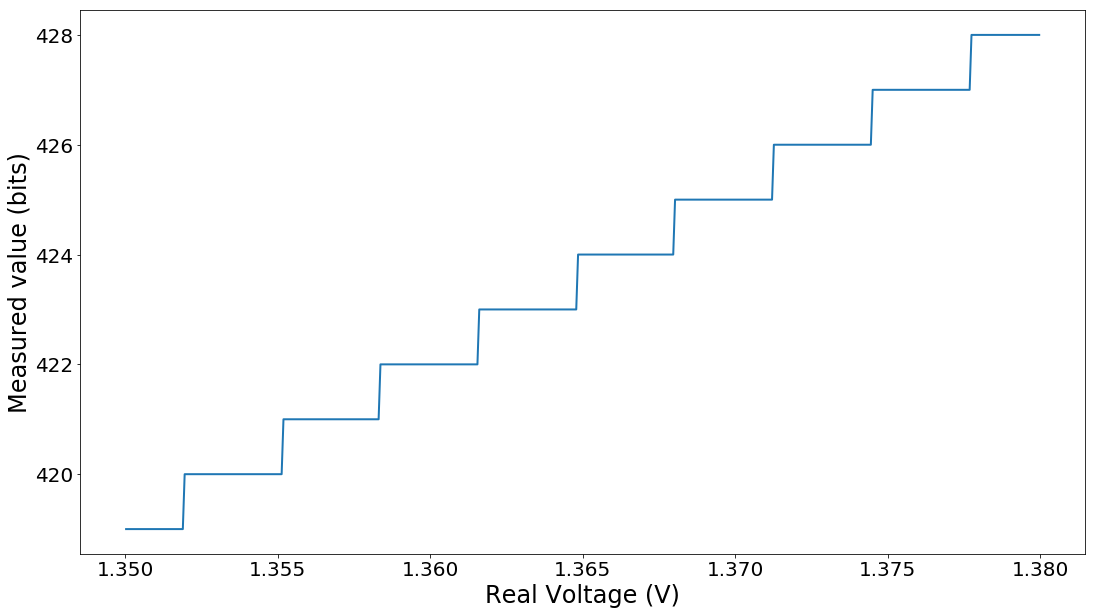
\includegraphics[width=.6\textwidth]{images/Chapter_03/digitalization.png}
\end{center}

The figure above shows a detail of how the digitalization looks like for a range of voltages. You see the discrete steps that the digital value takes for different voltages. Digitizing signals is a very important topic for anybody working in the lab. There are a whole set of ramifications regarding visualization, data storage and more. 

Particularly, the {PFTL DAQ} has a different behavior for reading than for setting values. The output channels take $4095$ ($2^{12}-1$) different values, i.e. they work with 12 bits instead of 10. Knowing the number of bits, also allows us to calculate the minimum difference between two output values:

\begin{equation}
 \frac{3.3\,\textrm{V} - 0\,\textrm{V}}{4096} \approx 0.0008\,\textrm{V} = 0.8\,\textrm{mV}
\end{equation}

The equation above shows you how the resolution of your experiment is affected by the digitalization of the signals. You will not be able to create voltages with a difference between them below $0.8\,\textrm{mV}$, and you won't be able to detect changes below $3\,\textrm{mV}$. Later in the book, we will come back to this discussion when you need to decide some parameters for visualizing your data. 

Keep in mind that digitizing is everywhere. Digital cameras have a certain \emph{bit depth}, which tells you which range of values they can cover, i.e. their dynamic range. Oscilloscopes, function generators, acquisition cards, they all have a certain digital resolution. You will always be sure that the resolution you get is enough to observe the properties you are interested in. 

\section{Doing an experiment}
Up to now, we have developed everything that we need to actually measure the current that goes
through the light emitting diode, you only need to combine setting an analog
output and then reading an analog input.

\exercise{Write a method that allows you to linearly increase an analog output in a given range of values for a given number of steps. Don't forget to add a delay
between each update.}

\exercise{Write a method that is able to record a given analog input while an
analog output increases linearly.}

\exercise{Make a plot of your results.}

Doing an experiment at this stage is left as an exercise to the reader. In the following chapter, we are going to see how to perform experiments in a much more flexible way. If you try to solve the exercises, you will see that by having classes, your code is much more reusable.
It is very easy to share with a colleague that has the same device, and
it can be adapted and expanded. You also should keep in mind that when
working with devices, it may very well be that someone else has already
developed a Python driver for it, and you can just use it. One of the
keys to developing sustainable code is to compartmentalize different
aspects of it. Don't mix the logic of a special experiment with the
capabilities of a device, for example.

\textbf{Remember the Onion}: We have discussed in the Introduction, that
one should always remember the onion principle when developing. If you
see the outcome of the exercises you just finished, you will notice that
you are failing to follow the principle. You have added a lot of
functionality to the driver class that does not reflect what the device
itself can do. The {PFTL DAQ} doesn't have a way of linearly
increasing an output, you have achieved that extra behavior with a loop
in a program. If you start transferring the logic of your own experiment
to the driver class, you will start creating a gigantic class that
others will not be able to (re-)use.

When developing software, especially when dealing with devices, one has
to separate what the device can do and what extended functionality we
can achieve. A scan of an analog output is a consequence of sequential changes of a value,
and therefore we should have those ideas in a different portion of the code. In the beginning, it may be very hard to realize what is the true reason for separating the code like this, but with time it will become clearer. When you develop the driver
for a device, such as what we have been doing in this chapter, we have to keep as close as possible to what the manual specifies. 

\section{Using PyVISA}\label{section:pyvisa}
What we did in the previous section is very interesting, but as you may have guessed, we are not the first ones who want to achieve the same. Plus, you may ask yourself what happens if you have a device that can communicate through different connections, not only serial. You will have to develop a new driver for each one and that is not handy. 

Even if not super well known, there is a standard developed by a consortium of companies called \href{https://en.wikipedia.org/wiki/Virtual_instrument_software_architecture}{Virtual instrument software architecture}, or VISA for short. This standard allows communicating with devices independently from the communication channel selected. There are different backends developed, including the one of National Instruments and Tektronix. They are hard to install and do not work on every operating system. 

There is also a pure Python implementation of VISA called \mintinline{python}{pyvisa-py} which is still work in progress but for simple devices like the {PFTL DAQ} it should be enough. We will show you in this section how to get started with pyvisa-py, but it is not a requirement of the book. You can use it as a reference for later in your projects. 

First, you need to install two libraries, \mintinline{python}{pyvisa} and \mintinline{python}{pyvisa-py}:

\begin{minted}{bash}
 pip install pyvisa
\end{minted}

And then, you can install the backend:

\begin{minted}{bash}
 pip install pyvisa-py
\end{minted}

If you are working on a clear environment, you will also need to install PySerial since it is not marked as a dependency of pyvisa-py. And now, you can start using it. Let's start in a python interpreter directly, before going to more complex code. Visa allows you to list your devices:

\begin{minted}{pycon}
 >>> import visa
 >>> rm = visa.ResourceManager('@py')
 >>> rm.list_resources()
 ('ASRL/dev/ttyACM0::INSTR',)
 >>> dev = rm.open_resource('ASRL/dev/ttyACM0::INSTR')
 >>> dev.query('IDN\n')
 'General DAQ Device built by Uetke. v.1.2017\n'
\end{minted}

If you follow the code, you can see that after importing \mintinline{python}{visa}, we start the resource manager specifying that we want to use the Python backend. If you have any other backend installed on your computer, this is the place to define it. Then, we list all the devices connected to the computer. Bear in mind that this will depend on the other packages that you installed. For example, we have only PySerial, and therefore pyvisa-py will only list serial devices. You can install PyUSB in order to work with USB devices, etc. The rest of the code is very similar to what we have done before.

Pay attention to the \mintinline{python}{query} method that we use to get the serial number from the device. We didn't develop it. PyVISA already took care of defining query for us. Not only PyVISA takes care of the query method, but they have plenty of options that you can use, such as transforming the output according to some rules, establishing the write termination, etc. If you were to follow the pyVISA path, you can start by reading \href{https://pyvisa.readthedocs.io/en/master/index.html}{their documentation}.

\textbf{Why didn't we start with pyVISA?}. There are several reasons. One is pedagogical. It is better to start with as few dependencies as possible, so you can understand what is actually going on. Now you know exactly what commands need to be sent, you are aware of the encoding and line termination. You are also aware of the fact that to read from the device, you first have to write something to it. The other reason is practical. PyVISA works great with the National Instruments backend, but it is hard to install. Pyvisa-py is still slightly work in progress and to keep the consistency of the book through time, it was better not to ask it as a dependency. 

Once you gain confidence with the topics covered in this chapter, you will be able to explore other solutions and alternatives.

\section{Introducing Lantz}\label{section:lantz}
Defining a class for your device was a very big step in terms of
usability. You can easily share your code with your colleagues and
they can immediately start using what you have developed with really few extra lines of code. However, as soon as you want to develop drivers for a new
device, you will find yourself repeating a lot of the things you have
done right now. Setting the line ending, the encoding, etc. And it only
works for serial devices, when you want to add a {USB} or {GPIB} device
you will have to re-think everything.

Moreover, there are more sophisticated properties that can be improved.
For example, you could use some cache in order to avoid reading too
often from a busy device or re-setting a property that didn't change. We
could also set some limits, for example to the analog output values. Imagine that you have a device that can handle up to $2.5\,\textrm{V}$. If you set the analog output to
$3\,\textrm{V}$ you would burn it. 

Fortunately, there are packages that were written especially to address this kind of problems. We are going to mention only one because it is
a project with which we collaborate: \href{https://github.com/lantzproject/lantz}{Lantz}. You can install it
by running:

\begin{minted}{bash}
pip install lantzdev
\end{minted}

\note{We introduce Lantz here for you to see that there is a lot of room for
improvement. However, through this book, we are not going to use it, and
that is why it was not a requirement when you were setting up the
environment. Lantz is under development and therefore some of the
fine-tuned options may not work properly on different platforms. Using
Lantz also shifts a lot of the things you need to understand
under-the-hood and it is not what we want for an introductory course. If
you are interested in learning more about Lantz and other packages, you
should check for the Advanced Python for the Lab book when you are
finished with this one.}

Lantz is a Python package that focuses exclusively on instrumentation. We strongly suggest you check their documentation and tutorials since they
can be very inspiring. Here we will just show you how to write your own
driver for the {PFTL DAQ} device using Lantz, and how to take
advantage of some of its options. Lantz can do much more than what we show you here, but with these basics, you will be able to start in the
proper direction.

Let's first re-write our driver class to make it Lantz-compatible, we
start by importing what we need and define some of the constants of our
device. We will also add a simple method to get the identification of the
device. Note that the first import is a \mintinline{python}{MessageBasedDriver},
exactly what we have discussed at the beginning of the chapter.

\begin{minted}{python}
from lantz.messagebased import MessageBasedDriver
from lantz import Feat

class MyDevice(MessageBasedDriver):

    DEFAULTS = {'ASRL': {'write_termination': '\n',
                        'read_termination': '\n',
                        'encoding': 'ascii'
                        }}

    @Feat()
    def idn(self):
        return self.query('IDN')

if __name__ == "__main__":
    dev = MyDevice.via_serial('/dev/ttyACM0')
    print(dev.idn)
\end{minted}

There are several things to point out in this example. First, we have to
note that we are importing a very special module from Lantz, the
\mintinline{python}{MessageBasedDriver}. Our class \mintinline{python}{MyDevice} inherits from the
\mintinline{python}{MessageBasedDriver}. If you are unsure of what inheriting means,
I suggest you check the appendix \ref{classes-in-python}. Surprisingly, there is
no \mintinline{python}{__init__} method in the snippet above. The reason for this is that the instantiation of the class is different, as we will see later. The first thing we do is to
define the \mintinline{python}{DEFAULTS} of our class. At first sight, you probably
see that they really look the same to the ones we have defined for our own driver. The \mintinline{python}{ASRL} option is for serial devices. In principle, you can specify different defaults for the same device depending on the connection type. If you were using a {USB} connection, you would
have used \mintinline{python}{USB}, or \mintinline{python}{GPIB} instead of, or in
addition to, \mintinline{python}{ASRL}.

The only method that we have included in the example is \mintinline{python}{idn} because,
even if simple, it already shows some of the most interesting
capabilities of Lantz. First, you can see that we have used \mintinline{python}{query} instead
of \mintinline{python}{write} and \mintinline{python}{read}. Indeed, Lantz depends on pyVISA, so what is happening here is that under the hood, you are using the same command that we saw in the previous section. Bear in mind that the write and read termination are automatically used by Lantz. 

An extra syntactic thing to note is the \mintinline{python}{@Feat()} before the
function. It is a \mintinline{python}{decorator}, one of the most useful ways of
systematically altering the behavior of functions without rewriting.
Without entering too much into details, a decorator is a function that
takes as an argument another function. In Lantz, when using a
\mintinline{python}{Feat}, it will check the arguments that you are passing to the
method before actually executing it. Another advantage is that you can treat the method as an attribute. For example, you will be able to do something like this
\mintinline{python}{print(dev.idn)} instead of \mintinline{python}{print(dev.idn())} as we did
in the previous section.

\exercise{Write another method for getting the value of an analog input. 
Remember that the function should take one argument: the channel.}

In order to read or write to the device, you need to define new methods.
If you are stuck with the exercise, you can find inspiration from the
example on how to write to an analog output below.

\begin{minted}{python}
output0 = None

[...]

@Feat(limits=(0,4095,1))
def set_output0(self):
    return self.output0

@set_output0.setter
def set_output0(self, value):
    command = "OUT:CH0:{}".format(value)
    self.write(command)
    self.output0 = value
\end{minted}

What we have done may end up being a bit confusing for people working with
Lantz and with instrumentation for the first time. When we use
\mintinline{python}{Features} in Lantz, we have to split the methods in two: first a
method for getting the value of a feature and then a method for setting
the value. Since our device doesn't have a way of knowing the value that
an output was set to, we have to trick it a bit. When we initialize the
class, we will have an attribute called \mintinline{python}{output0}, with a
\mintinline{python}{None} value. Every time we update the value of the output on
channel 0, we are going to store the latest value in this variable.

The first method is for reading the value from the device, pretty much
in the same way than with the \mintinline{python}{idn} method. The main difference
here is that we are specifying some limits to the options, exactly as
the manual specifies for the {PFTL} device. The method
\mintinline{python}{set_output0} returns the last value that has been set to the
channel 0, or \mintinline{python}{None} if it has never been set to a value. When
you use \mintinline{python}{@Feat} in Lantz, we are always forced to define the
first method, also called a \mintinline{python}{getter}. This is why we have to
trick Lantz and we couldn't simply define the \mintinline{python}{setter}. On the
other hand, if the setter is not defined, it means that you have a
read-only feature, such as with \mintinline{python}{idn}. The second method
determines how to set the output and has no return value. The command is
very similar to how the driver you developed earlier works. Once you
instantiate the class, the two commands can be used like this:

\begin{minted}{python}
print(dev.set_output0)
dev.set_output0 = 500
print(dev.set_output0)
\end{minted}

Even if the programming of the driver was slightly more involved, you
can see that the results are very clear. A property of the real device
appears also as a property of the Python object. Remember that when you
execute \mintinline{python}{dev.set_output0 = 500} you are really changing an
output in your device. The line looks very innocent, but it isn't. A lot
of things are happening under the hood both in Python and on your
device. I encourage you to see what happens if you try to set a value
outside of the limits of the device, i.e., try something like
\mintinline{python}{dev.set_output0=5000}.

You may have noticed that the method works only with the analog output
0; this means that if you want to change the value of another channel,
you will have to write a new method. This is both unhandy and starts to
violate the law of the copy/paste. If you have a device with 64
different outputs it would become incredibly complicated to achieve a
simple task. Fortunately, Lantz allows you to program such a feature
with not too much effort:

\begin{minted}{python}
output = [None, None]

[...]

@DicFeat(keys=[0, 1], values=(0, 4095, 1))
def output(self, key):
    return self.output[key]

@output.setter
def output(self, key, value):
    self.write('OUT:CH{}:{}'.format(key, value))
\end{minted}

Because the {PFTL DAQ} device has only two outputs, we initialize a
variable \mintinline{python}{output} with only two elements. The main difference
here is that we don't use a \mintinline{python}{Feat} but a \mintinline{python}{DicFeat}, which
will take two arguments instead of one: the channel number and the
value. The \mintinline{python}{keys} are a list containing all the possible options
for the channel. The
values, as before, are the limits of what you can send to the device. 
the last \mintinline{python}{1} is there just to make it explicit that we take
values in steps of 1. You can use the code in this way:

\begin{minted}{python}
dev.output[0] = 500
dev.output[1] = 1000
print(dev.output[0])
print(dev.output[1])
\end{minted}

And now it makes much more sense and it is cleaner. You can also check
what happens if you set a value outside of what you have established as
limits. The examples above only scratch the surface of what Lantz can
do. It is strongly suggested that you check
\href{http://lantz.readthedocs.io}{their website} and follow the guides
and examples. Even if you don't use Lantz for your driver, you can get a
lot of inspiration regarding how to work with your code and how to
improve your programming strategies. We have covered how to set an
analog output because it was the hardest task. You can do the
following exercise:

\exercise{Write a \texttt{@DictFeat} that reads a value of any given analog 
input channel.}

\note{Lantz does a great work working with units as well. If you read the 
documentation, you will see that you can specify the units directly in
the \mintinline{python}{@Feat} and Lantz will take care of the conversions to the
natural units of your device. It will also check that the input is
within the limits you have specified.}

\section{Conclusions}\label{section:conclusions}
In this chapter, we have covered a lot of details regarding the
communication with devices, how to start writing and reading from a
device at a low level, straight from Python packages such as
\emph{PySerial}. We have also seen that it is handy to develop classes
and not only plain functions or scripts. We have briefly covered pyVISA and Lantz,
two Python packages that allow you to build drivers in a systematic, clear
and easy way. The rest of the book doesn't depend on them, but it is important that you know of their existence. 

It is impossible in a book to cover all the possible scenarios that you
are going to observe over time in the lab. You may have devices that
communicate in different ways, you may have devices that are not
messaged based, etc. The important point, not only in this chapter but
also throughout the book, is that once you build a general framework in
your mind, it is going to be much easier to find answers online and to
adapt others' code.

Remember, documentation is your best friend in the lab. You always have
to start by checking the manual of the devices you are using. Sometimes some manufacturers already provide drivers for Python. Such is the case of National Instruments and Basler, but they are not the only ones. Checking the manuals is also crucial because you have
to be careful with the limits of your devices. Not only to prevent damages to devices but also because if you employ an instrument
outside of the range for which it was designed, you can start generating
artifacts in your data. When in doubt, always check the documentation of the
packages you are using. PySerial, PyVISA, PyUSB, Lantz, they are quite complex
packages and they have many options. In their documentation pages, you
can find a lot of information and examples. Moreover, you can also check
how to communicate with the developers because they are very often able to give you a hand with your problems. 

\section{Addendum 1: Unicode Encoding}\label{section:unicode}
We have seen in the previous sections that when you want to send a message to the device, you need to transform a string to binary. This is called encoding a 
string. As you may be aware, computers do not understand what is a letter, they just understand binary information, 1s and 0s. This means that if you want to display an \texttt{a}, or a \texttt{b}, you need to find a way of converting a 
character into bytes and the other way around. 

A standard that appeared several years ago is called ASCII, which you may have already heard of. ASCII contemplates transforming 128 different characters to binary. Remember that characters also include marks such as \texttt{!} or 
\texttt{:}, and numbers. 128 is not a random number, it is $2^7$. For the English language, 128 characters are enough. But for languages such as Spanish, which have characters like \texttt{ñ}, French with its different accents, and without even mentioning languages that use a non-latin script, forced the appearance of new standards. 

As you can imagine, having more than one \textit{standard} is incompatible with the definition of a standard. Imagine that you write a text in French, using a special encoding, and then you share it with someone else. That other person does not know which encoding you used and decides to decode it using a Spanish standard. 
What will the output be? Very hard to know, and probably very hard to read by a person. 
Remember that this doesn't even consider the possibility of having text 
written in a non-latin script such as Russian or Chinese.

If you are old enough, you may remember that some websites were not rendering correctly, and it was very common to find weird characters on e-mails. This was all due to the mess that different string encodings generated. I even remember that some web hosting companies did not allow hosting Chinese websites because of the overhead that decoding Chinese characters imposed on the servers. This unbearable situation gave rise to a new encoding standard called, as you guessed, 
\textbf{Unicode}. 

Unicode uses the same definition than ascii for the first 128 characters. Which means that any ascii document will look exactly the same if decoded with 
Unicode. The advantage is that Unicode defines encoding for millions of extra characters. This includes all the modern scripts, but also ancient ones such as 
Egyptian hieroglyphs, allowing people to exchange information without problems. Unicode is also the standard for most emojis with which you may be very familiar. 

Thus, when we want to send a command to a device such as the {PFTL DAQ}, we need to determine how to encode it. Most devices work with ASCII values, but since they overlap with the 
Unicode standard, there will be no conflict. Bear in mind that devices manufactured outside of the US may also use characters beyond the first 128, and thus choosing Unicode over ascii is always an advantage. In Python, if you want 
to choose how to encode a string, you can do the following:

\begin{minted}{python}
 var = 'This is a string'.encode('ascii')
 var1 = 'This is a string'.encode('utf-8')
 var2 = 'This is a string with a special character ñ'.encode('utf-8')
\end{minted}

Utf-8 is the way of calling the 8-bit Unicode standard. The example above is quite self-explanatory. You may want to check what happens if on the last line you change \mintinline{python}{'utf-8'} by \mintinline{python}{'ascii'}. 

One of the changes between Python 2 and Python 3 that generated some headaches 
to unaware developers was the out-of-the-box support for Unicode. In Python 3 
you are free to use any utf-8 character not only in strings but also as 
variable names, while in Python 2 this is not the case. For example, this is 
valid in Python 3:

\begin{minted}{python}
 var_ñ = 1
\end{minted}

If you are curious to see how Unicode works, the Wikipedia article is very descriptive. Plus, the Unicode consortium keeps adding new characters based on the input not only from industrial leaders but also from individuals. You can see the latest emojis added and notice that some were proposed by local organizations that wanted to have a way of expressing their idiosyncrasies. 
